
\section{Proposed Method}

Penelitian ini mengusulkan kerangka kerja untuk mengembangkan sistem pelacakan invoice dan \textit{Proof of Delivery} (POD) yang mendukung penentuan prioritas pengiriman invoice. Kerangka kerja yang diusulkan mengintegrasikan proses akuisisi pengetahuan, formalisasi pengetahuan, pembangunan dataset, \textit{expert labeling}, serta pemodelan menggunakan pendekatan \textit{Rule-Based} dan Decision Tree C4.5.

Gambar~\ref{fig:research_framework} menunjukkan alur penelitian yang diusulkan. Proses dimulai dari akuisisi pengetahuan yang diperoleh dari regulasi pelanggan, data historis invoice, dan pengetahuan pakar. Pengetahuan tersebut kemudian diformalkan menjadi aturan operasional dan atribut penelitian untuk membangun dataset. Dataset yang telah diberi label oleh pakar selanjutnya digunakan untuk membangun model \textit{Rule-Based} dan Decision Tree C4.5. Kedua model kemudian dievaluasi dan dibandingkan menggunakan metrik klasifikasi untuk menentukan pendekatan yang paling sesuai dalam penentuan prioritas pengiriman invoice.

\begin{figure}[htbp]
\centering
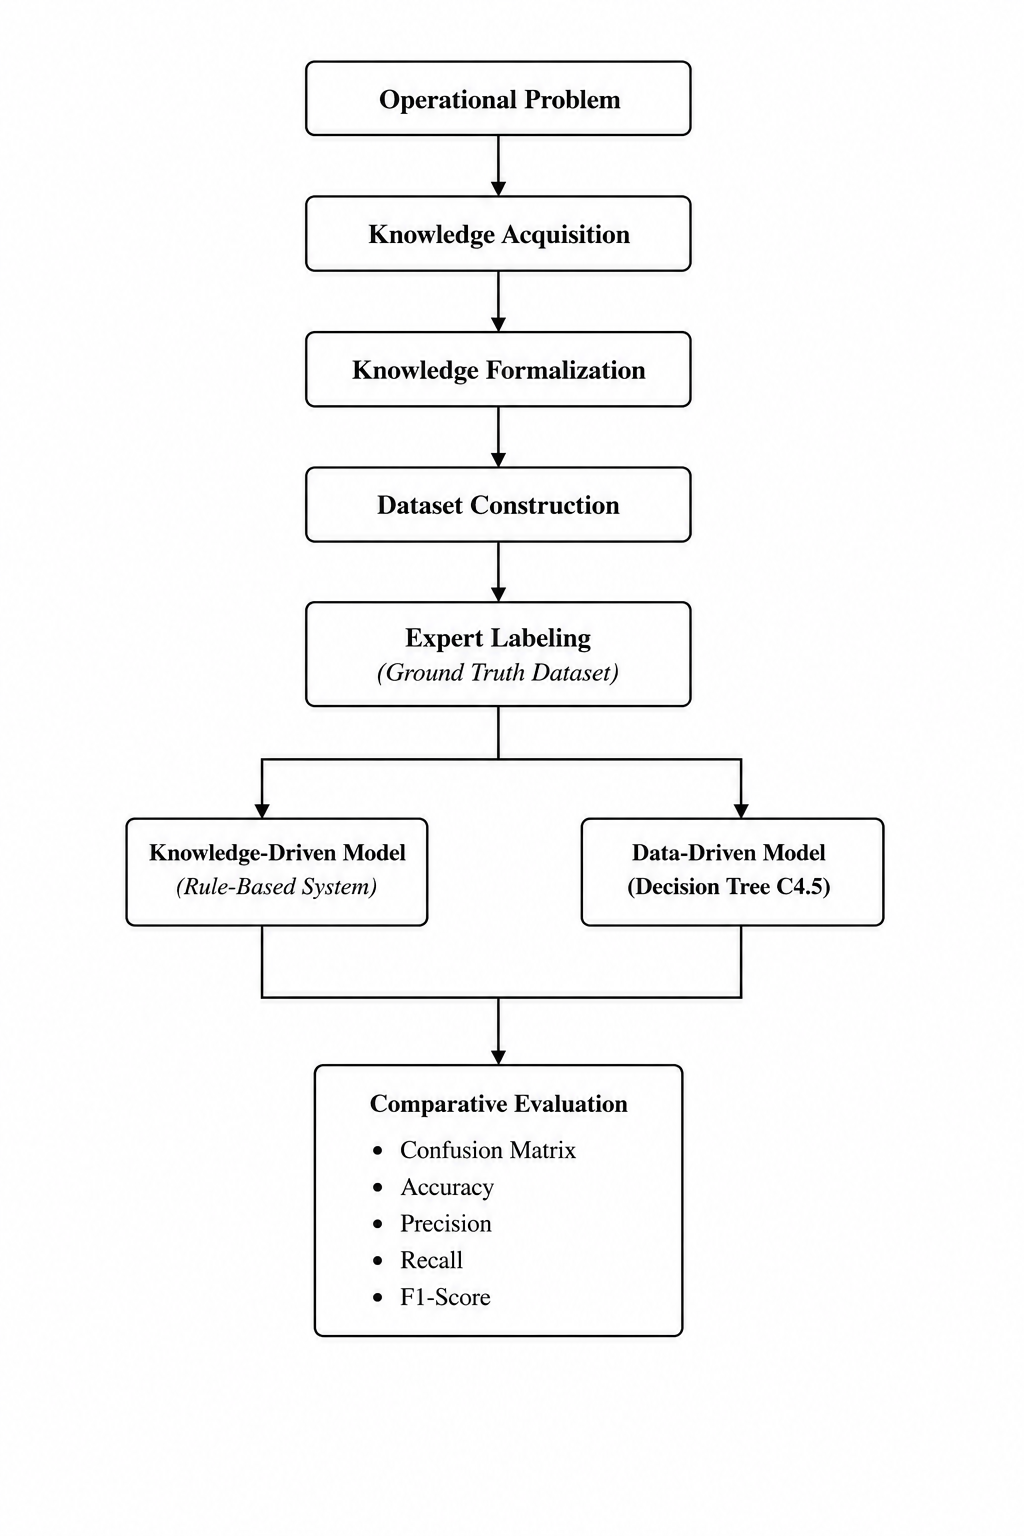
\includegraphics[width=0.82\columnwidth]{research_framework-1.png}
\caption{Proposed Research Framework}
\label{fig:research_framework}
\end{figure}

Tahapan pada kerangka penelitian tersebut dijelaskan secara rinci pada bagian \textit{Knowledge Acquisition}, \textit{Knowledge Formalization}, \textit{Dataset Construction}, \textit{Expert Labeling}, pembangunan model \textit{Rule-Based}, pembangunan model Decision Tree C4.5, serta evaluasi komparatif.

```latex
\subsection{Knowledge Acquisition}

Tahap \textit{Knowledge Acquisition} bertujuan untuk mengidentifikasi dan mengumpulkan pengetahuan operasional yang digunakan dalam proses penentuan prioritas pengiriman invoice. Pada penelitian ini, pengetahuan tidak hanya diperoleh dari data historis, tetapi juga dari aturan operasional pelanggan dan pengalaman staf administrasi. Seluruh informasi yang diperoleh pada tahap ini menjadi dasar dalam proses \textit{Knowledge Formalization} untuk membangun aturan keputusan dan atribut penelitian.

\subsubsection{Customer Regulation}

Regulasi pelanggan merupakan sumber pengetahuan eksplisit yang menjelaskan aturan administrasi setiap pelanggan. Informasi yang dikumpulkan meliputi jenis \textit{cut-off}, nilai \textit{cut-off}, jadwal penerimaan invoice, serta hari operasional penerimaan dokumen. Aturan tersebut digunakan untuk memahami karakteristik operasional masing-masing pelanggan dan menjadi acuan dalam proses penentuan prioritas pengiriman.

\subsubsection{Historical Invoice Data}

Data historis invoice digunakan untuk menggambarkan aktivitas operasional perusahaan yang sebenarnya. Dataset ini memuat informasi seperti nomor invoice, pelanggan, tanggal penerimaan invoice, tanggal pengiriman, dan riwayat distribusi. Data historis digunakan untuk mengidentifikasi pola pengiriman invoice sekaligus menjadi dasar dalam proses pembangunan dataset penelitian.

```latex
\subsubsection{Expert Knowledge}

Selain data operasional, penelitian ini juga memanfaatkan pengetahuan dari staf administrasi yang berpengalaman dalam menentukan prioritas pengiriman invoice. Pengetahuan tersebut digunakan untuk mengidentifikasi pertimbangan operasional yang belum terdokumentasi serta menyusun pedoman \textit{expert labeling}.

Hasil dari tahap \textit{Knowledge Acquisition} adalah kumpulan pengetahuan operasional yang diperoleh dari regulasi pelanggan, data historis invoice, dan pengetahuan pakar. Ringkasan sumber pengetahuan, informasi yang dikumpulkan, dan tujuan penggunaannya disajikan pada Tabel~\ref{tab:knowledge_acquisition}. Selanjutnya, pengetahuan tersebut digunakan sebagai masukan pada tahap \textit{Knowledge Formalization} untuk membentuk atribut penelitian dan aturan keputusan yang digunakan dalam proses pemodelan.

\begin{table}[htbp]
\caption{Knowledge Sources in the Knowledge Acquisition Stage}
\label{tab:knowledge_acquisition}
\centering
\renewcommand{\arraystretch}{1.2}
\resizebox{\columnwidth}{!}{
\begin{tabular}{|p{0.22\columnwidth}|p{0.32\columnwidth}|p{0.32\columnwidth}|}
\hline
\textbf{Knowledge Source} &
\textbf{Collected Information} &
\textbf{Purpose} \\
\hline

Customer Regulation &
Cut-off policy, cut-off value, receiving schedule, receiving day &
Capture explicit operational rules for each customer. \\
\hline

Historical Invoice Data &
Invoice number, customer, receive date, delivery date, delivery history &
Represent historical operational activities and support dataset construction. \\
\hline

Expert Knowledge &
Priority criteria, operational considerations, delivery decision strategy &
Develop labeling guidelines and validate operational rules. \\
\hline

\end{tabular}
}
\end{table}
```
